\begin{prob}

\end{prob}

\begin{sol}


من راستش نمیدونستم هر ستونی دقیقا معنیش چیه و بیشتر اونهایی که میدونستم معنیش چیه و ممکنه کمک کنه را نگه داشتم.
تعدادی از ستون ها را با 0  پر کردم. و بعدش اونایی که مقدار NAN زیادی بیشتر از 0.8 داشت را حذف کردم.  سپس بقیه را با 0  دوباره جایگذاری کردم. 
GOALS از مهمترین ستون ها می باشد چرا که برای مثال دروازه زبان ها یا مدافعان تعداد گل کمتری به ثمر رساندند و این برای مهاجهم ها برعکس و مقدار زیادی است.
یا مثلا CS فقط برای دروازه زبان است. کرنرها نیز موارد مهمی هستند که بازیکنان جلویی بیشتر آن را می‌زنن، همچنین سانت‌ها نیز. تقریبا بیشتر فیلدها مهم هستند و بیشتر مهم است که چگونه با ان ها رفتار شود و مقدار Nan آن ها با چه مقدار مناسبی پر شود.


بخش ۵)
ابتدا اثبات می‌کنیم که k-means به صورت یکنواخت  
 $\psi\left(X^{(t)}\right)=\frac{1}{n} \sum_{j=1}^{K} \sum_{i=1}^{n}\left\|x_{i}, c_{j}\right\|^{2}$
را کاهش می‌دهد که  
 $X^{(t)}$ 
تقسیم بندی فعلی 
 $X_{1}^{(t)}, \ldots, X_{K}^{(t)}$ 
با
centroid 
های 
$c_{1}^{(t)}, \ldots, c_{K}^{(t)}$ 
است.
در هر مرحله از اجرای الگوریتم ،k-means $\mathcal{A}\left(x_{i}\right)$ به صورت
$
\mathcal{A}\left(x_{i}\right) \longleftarrow \underset{j \in\{1, \ldots, K\}}{\arg \min }\left\|x_{i}-c_{j}\right\|^{2}$
تعریف می‌شود.
که به $\mathcal{A}^{(t)}$، تابع انتساب گفته می‌شود.
در این صورت از آنجا که $\mathcal{A}\left(x_{i}\right)$ مقدار $\left\|x_{i}-c_{j}\right\|^{2}$ را روی همه $j \in\{1, \ldots, K\}$ کمینه می‌کند و $c_{j}^{(t+1)}$  نیز مقدار $\left\|x_{i}-c_{j}\right\|^{2}$ را روی همه $x_{i} \in X_{j}$ کمینه می‌کند، خواهیم داشت:
$$
\psi\left(X^{(t)}\right) \geqslant \sum_{j=1}^{K} \sum_{x_{i} \in X_{j}^{(t)}}\left\|x_{i}, c_{\mathcal{A}_{\left(x_{i}\right)}^{(t+1)}}^{(t)}\right\|^{2}
$$

$$
\begin{array}{l}
\geqslant \sum_{j=1}^{K} \sum_{x_{i} \in X_{j}^{(t)}}\left\|x_{i}, c_{j}^{(t+1)}\right\|^{2} \\
\geqslant \psi\left(X^{(t+1)}\right)
\end{array}
$$

در این صورت اثبات می‌شود که این الگوریتم به طور یکنواخت مقدار
$\frac{1}{n} \sum_{j=1}^{K} \sum_{i=1}^{n}\left\|x_{i}-c_{j}\right\|^{2}$
را کاهش می‌دهد.

حال به اثبات صورت سوال گفته شده می‌پردازیم و تنها کافی است که نشان دهیم الگوریتم k-means پس از تعداد محدودی step متوقف می‌شود.
از انجا که تعداد محدودی تقسیم‌بندی وجود دارد و تعداد آن برابر
$ {N\choose k}$ 
است، در نتیجه دنباله 
$\psi\left(X^{(t)}\right)_{t \in \mathbb{N}}$
تعداد محدودی مقدار خواهد داشت. این بدین معناست که حالتی وجود دارد که  $\psi\left(X^{(t+1)}\right)=\psi\left(X^{(t)}\right)$
باشد و در نتیجه 
در step شماره $t$
‌داریم:
$X^{(t+1)}=X^{(t)}$
در غیر این صورت برخی از element ها اشتباه دسته‌بندی شده است.
در این اثبات صرفا یک باند نمایی برای مساله پیدا کردیم که نشان دهیم حتما در تعداد محدودی بار الگوریتم متوقف می‌شود.

بخش ۶)
از آنجا که استفاده از منابع اینرنتی در طول امتحان مجاز است من از مثال این 
\href{http://www.onmyphd.com/print.php?p=k-means.clustering}{link}
استفاده کردم.
هدف این لینک آن است که نشان دهد الگوریتم k-means در چه مثال‌هایی خوب عمل ‌می‌کند و در چه مثال‌هایی بد. 
اما من مثالی که در آن این صفحه از آن به عنوان مثال خوب یاد کرده است صرفا استفاده کردم و نتیجه‌گیری ها کاملا مشاهدات و استدلال‌های خودم است و تنها از اجرای آنلاین ان استفاده کردم.
همانگونه که در این صفحه گفته شده این مثالی است که در آن k-means به خوبی عمل می‌کند. اما اگر چندین بار الگوریتم را ران کنیم تا نقاطی که در ابتدا به عنوان نقاط تصادفی مرکز centroid ها initial می‌شود به گونه نامناسبی قرار گیرد و در نتیجه در ادامه اجرای الگوریتم در یک مینیمم محلی گیر می‌کند.
برای مثال در این شکل \ref{fig: 1} ما انتظار داشتیم که ۴ کلاستر به شکل زیر \ref{fig: 2} در آید اما انتخاب نقاط اولیه باعث شده در یک مینیمم محلی گیر کنیم.
و در نتیجه دو کلاستر پایینی با یکدیگر ادغام شده و یکی از کلاسترها به دو کلاستر تقسیم شود.
دلیل این امر نیز آن است که الگوریتم روی همه تقسیم‌بندی‌های یک تابع محدب نیست و در نتیجه خروجی به مقداردهی اولیه بستگی دارد. به همین منظور توصیه می‌شود گه چندین بار الگوریتم ران شود و خروجی مطلوب به عنوان جواب نهایی برداشته شود. 

\begin{figure}[h]
\centering
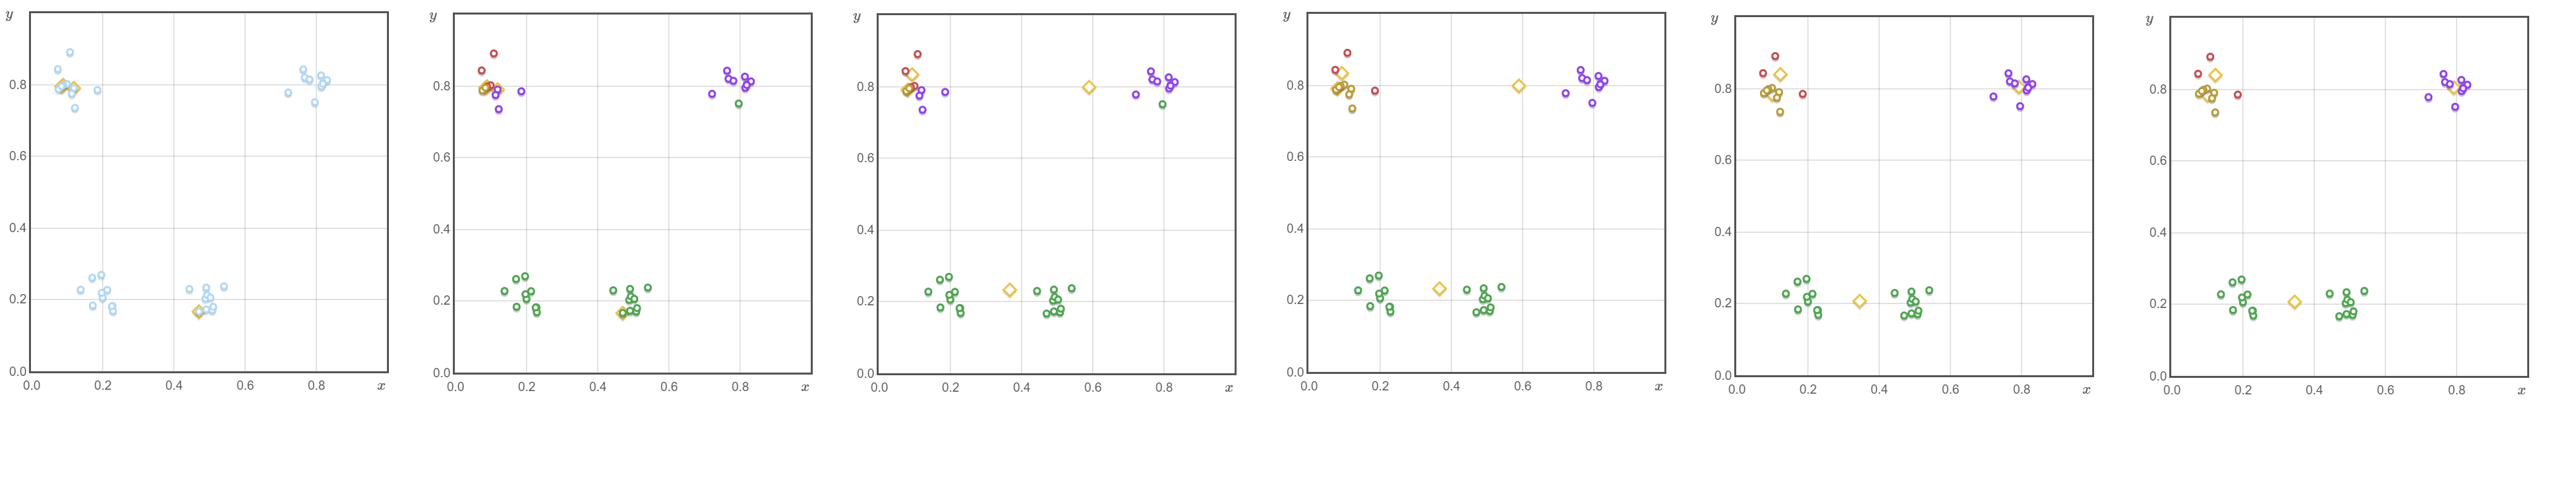
\includegraphics[scale=0.25]{1.png}
\caption{اجرای الگوریتم کلاسترینگ از سمت چپ به راست}
\label{fig: 1}
\end{figure}

\begin{figure}[h]
\centering
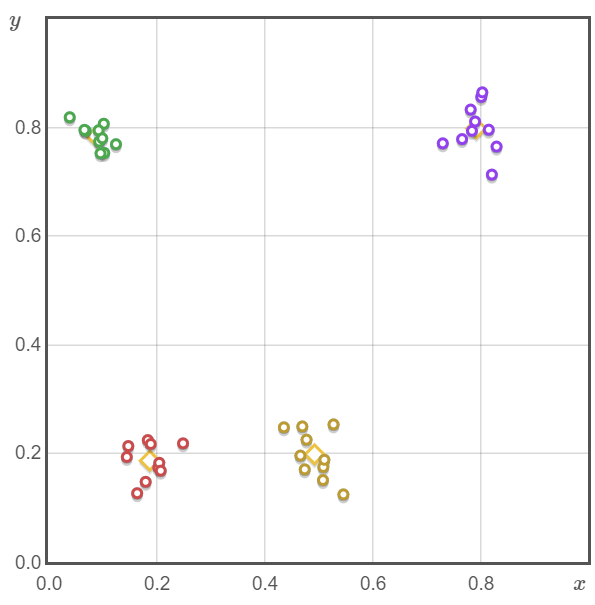
\includegraphics[scale=0.25]{2.PNG}
\caption{کلاسترینگ مطلوب}
\label{fig: 2}
\end{figure}


\end{sol}


\begin{prob}
\end{prob}
\begin{sol}

در نوتبوک به پیوست الگوریتم مقاله پیاده سازی شده است. در ادامه بحث می‌کنیم که الگوریتم این مقاله چگونه کار می‌دهد. 
اگر فرض کنیم که $U_{1}, U_{2}$ و ... به صورت iid بین 0 و 1 انتخاب شده باشند آنگاه اولین n ای که 
 $S_{n}=\sum_{i=1}^{n} U_{i} > 1 $
باشد را داشته باشیم.
انگاه $E(N)$ روی تمام n هایی که از این روش بدست امده بگیریم برابر e خواهد بود.
بنابراین یک تابع نوشتیم که n را برامون بدست بیاره و در نتیجه تعداد زیادی از اون‌ها را با هم جمع کنه از طریق reduce و در نهایت هم تقسیم بر تعداد جمع این اعداد را بکنیم.

\begin{figure}[h]
\centering
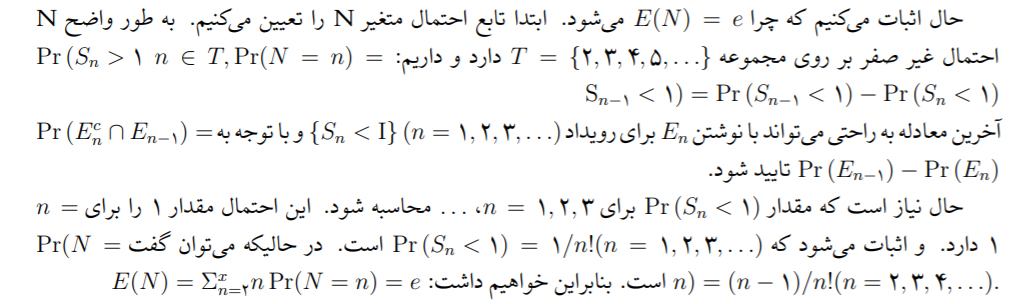
\includegraphics[scale=0.9]{555.PNG}
\end{figure}

\end{sol}

\begin{prob}
\end{prob}

\begin{sol}

قسمت اول) ابتدا به تعاریف می‌پردازیم و از روی تعاریف به نتیجه می‌رسیم. چه موقع یک FIS ماکسیمال است؟ اگر هیچ کدام از سوپرست های آن FIS دیگر پر تکرار نباشد و چه موقع یک FIS را بسته می‌نامیم؟ زمانی که هیچ سوپرستی از ان مقدار ساپورت برابر یا بزرگتری نداشته باشد.
پس یک مجموعه بسته می‌تواند سوپرستی پر تکرار داشته باشد اما شرط بسته بودن نقض نشود به زبانی دیگر سوپرست پرتکراری می‌تواند داشته باشد ولی آن سوپرست مقدار ساپورت برابر یا بزرگتری نداشته باشد. پس FIS ماکسیمال زیر مجموعه FIS بسته است. همچنین اگر از طریق برهان خلف نیز به این مساله نگاه شود و در نظر بگیریم که FIS ماکسیمال زیر مجموعه FIS های بسته نیست پس باید شرط آن را نقض کند در صورتی که مجموعه FIS ماکسیمالی نمی‌توان یافت که سوپرست آن از آن مقدار ساپورت برابر یا بزرگتری داشته باشد چرا که با ماکسیمال بودن FIS در تناقض است.


قسمت دوم) همانگونه که این موضوع در کلاس نیز بحث شد اگر به فرمول confidence نگاه کنیم کاملا متوجه آن خواهیم شد:

\begin{align*}
confidence (\{A \rightarrow B \}) =
\frac{support (\{A \rightarrow B \})}{support (\{A\})} = \frac{freq(A,B)}{frq(A)} = \mathrm{Pr} (B | A)
\end{align*}

اگر آیتمی از A  به B  اضافه شود آنگاه صورت کسر تغییر نخواهد کرد. اما ممکن است باعث شود که مخرج کسر بزرگتر شود (چرا که یک آیتم از مجموعه آن حذف شده است) و این موضوع باعث می‌شود مقدار confidence کاهش یابد و اگر تغییر نکند ثابت ماند که همان گزاره صورت سوال است.

قسمت سوم) بله از هر دو آن‌ها می‌توان استفاده کرد.
با توجه به قسمت اول می‌توان گفت که اگر سمت چپ rule یک عبارت ماکسیمال پرتکرار داشته باشیم آنگاه دیگر نیازی به بررسی سوپرست‌های آن نیست چرا که دیگر پرتکرار نیستند تا در سمت چپ قرار گیرند.
با توجه به قسمت دوم می‌توان rule هایی را که انتقال کالا باعث کم شدن confidence می‌شود را در صورتی که مقدار confidence آن‌ها از ترشولد کمتر می‌شود را در نظر نگرفت.

\end{sol}

\begin{prob}
\end{prob}
\begin{sol}

در قسمت ۱ با استفاده از کتابخانه pillow اقدام به بارگزاری عکس کردم و اندازه ان را چاپ کرده و کانال های مختلف رنگ را از یکدیگر نیز جدا کردم. در قسمت ۲ تابعی نوشتم که بتواند حاصلضرب اجزای مختلف svd را برای یک کانال حساب کند تا تصویر فشرده شده بدست آید. در قسمت ۳ برای بعد ۱۰۰ اقدام به محاسبه هر کانال کردم و در قسمت ۴ با استفاده از قسمت ۳ عکس کامل را ساختم این عکس را برای این پارامتر می‌توانید در شکل \ref{fig: 4-aprt4} مشاهده کنید.
این کار موجب شد عکس از ۷۱ به ۳۸ کیلوبایت فشرده شود. 
سپس در قسمت ۵، با گام ۱۰ از ۱ تا ۲۰۰ حرکت کردم و عکس‌های مختلف را ساختم. 
همانگونه که در نوتبوک میبینید دو عکس مربوط به پارامتر ۵۱ و ۶۱ را گذاشتم که با یکدیگر تفاوت خاصی (چشمی) ندارند و هر دو از کیفیت مناسبی برخوردار هستند.
بقیه عکس ها را می‌توانید در شکل \ref{fig:4} مشاهده کنید.
در قسمت ۶ حجم تک تک عکس ها را با کتابخانه os خواندم و نمودار مربوطه را کشیدم. 
همانجور که میبینید با اضافه شدن بعد حجم عکس نیز افزایش می‌یاید.
دلیل ان نیز کم تر حذف شدن دادگان در تابع فشرده ساز است که پارامتر dim ان را کنترل می‌کند.
در واقع می‌توان به جای این که مقدار $m*n*3$ تعیین کننده سایز نسبی عکس باشد، مقدار 
$ dim * (1+m+n) *3$
برابر سایز نسبی (بایت) عکس فشرده شده باشد. اولین عبارت حجم اصلی تصویر با ۳ کانال است که طول در عرض آن ضرب شده است. اما در دومی تنها برای ۳ کانال و ۳ ماتریس $U, Z, V$ اعداد ذخیره می‌شوند که تعداد اعداد غیر صفر آن‌ها برابر عبارت دوم است.
بدین صورت با افزابش $dim$ این مقدار افزایش می‌یابد که در نمودار نیز مشخص است. اما از یه جایی به می بینید که این نمودار شیبی کمتری پیدا می کند و از این فرمول حجم نسبی گفته شده کاملا پیروی نمی کند این به آن دلیل است که خود عکس وقتی به صورت jpg ذخیره می‌شود توسط jpg از یک نوع فشرده‌ساز استفاده می‌کند و نمودار خود jpg خود نیز به شکل جذری است .

برای قسمت ۷، طبق اسلاید باید انرژی ماتریس sigular-value در هر یک از حالت ها محاسبه شود و پارامتر بعد مناسب به نحوی انتخاب شود که حداقل ۹۰ درصد از انرژی را در خود داشته باشد.
کد این قسمت نیز مانند بقیه قسمت ها در نوتبوک زده شده است و مقدار این فاصله انرژی با حد $0.001$  مقدار انرژی محاسبه شده است. این مقدار dim برای هر یک از کانال ها به صورت مجزا حساب شده و سپس max آن در نظر گرفته شده است تا مقدار حد مورد نظر تضمین شود. 

همچنین راهکار دیگری که به ذهنم می‌رسد این است که ما دوست داریم حجم فایل ها کم شود در عین حالت ارور بین عکس فشرده شده و عکس اصلی نیز کم باشد. 
با افزایش مقدار dim مشاهده می‌کنیم که این خطا کاهش می یابد اما در عوض حجم افزایش پیدا می کند ( شکل خطا در بخش اخر نوتبوک کشیده شده است). 
در این صورت می توان یک تابع هدف تعریف کرد که با توجه به مقدار خطا و مقدار حجم فایل برای ما مقدار dim مناسب را پیدا کند. 
این تابع هدف دارای دو پارامتر مقدار خطا و حجم فایل در هر dim است که با استفاده از ۲ ضریب مثبت باید کمینه شود.
هر کدام از ضریب ها در جه اهمیت مد نظر ما را برای هر پارامتر بیان می‌کند.


\begin{figure}[h]
\centering

\includegraphics[scale=0.2]{part4.jpg}
\caption{بعد ۱۰۰}
\label{fig: 4-aprt4}
\end{figure}


\begin{figure}[h]
    \begin{minipage}[t]{.24\textwidth}
        \centering
        
\includegraphics[width=1.1\textwidth]{1.jpg}
        \subcaption{ابعاد ۱}\label{fig:p1}
    \end{minipage}
    \hfill
    \begin{minipage}[t]{.24\textwidth}
        \centering
        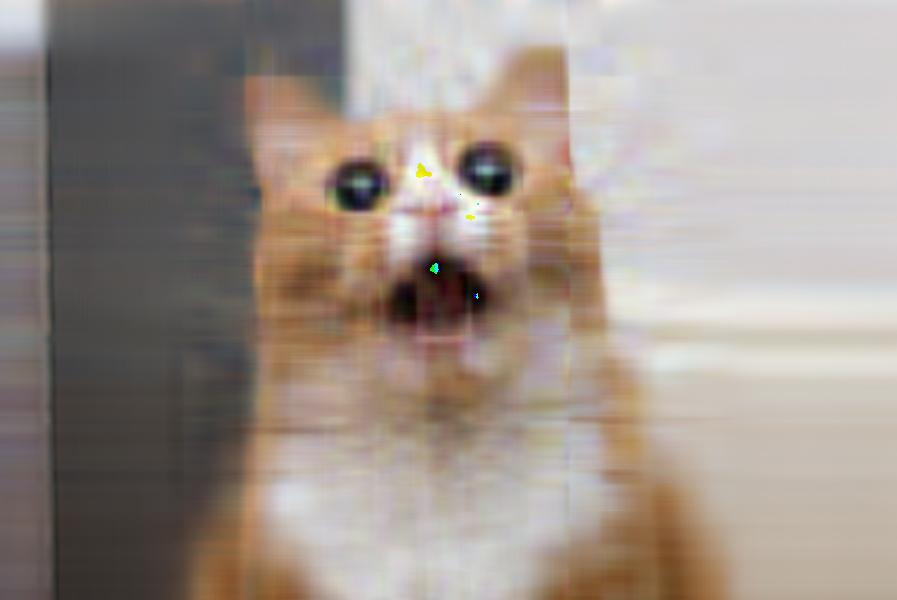
\includegraphics[width=1.1\textwidth]{11.jpg}
        \subcaption{ابعاد ۱۱}\label{fig:p11}
    \end{minipage}  
    
            \begin{minipage}[t]{.24\textwidth}
        \centering
        
\includegraphics[width=1.1\textwidth]{21.jpg}
        \subcaption{ابعاد ۲۱}\label{fig:p21}
    \end{minipage}
    \hfill
    \begin{minipage}[t]{.24\textwidth}
        \centering
        
\includegraphics[width=1.1\textwidth]{31.jpg}
        \subcaption{ابعاد ۳۱}\label{fig:p31}
    \end{minipage}  

    \begin{minipage}[t]{.24\textwidth}
        \centering
        
\includegraphics[width=1.1\textwidth]{41.jpg}
        \subcaption{ابعاد ۴۱}\label{fig:p41}
    \end{minipage}
    \hfill
    \begin{minipage}[t]{.24\textwidth}
        \centering
        
\includegraphics[width=1.1\textwidth]{51.jpg}
        \subcaption{ابعاد ۵۱}\label{fig:p51}
    \end{minipage}  
    
    \begin{minipage}[t]{.24\textwidth}
        \centering
        
\includegraphics[width=1.1\textwidth]{61.jpg}
        \subcaption{ابعاد ۶۱}\label{fig:p61}
    \end{minipage}
    \hfill
    \begin{minipage}[t]{.24\textwidth}
        \centering
        
\includegraphics[width=1.1\textwidth]{71.jpg}
        \subcaption{ابعاد ۷۱}\label{fig:p71}
    \end{minipage} 
    \caption{شکل ها با پارامترهای مختلف بعد} 
    \label{fig:4}
\end{figure}

\end{sol}